\subsection{Subtracting Amplifier:}

Once the circuit in Figure 3.5.0 were assembled, we connect the respectively sources in terminals 7 and 4, then with the voltmeter we measure both input voltages $V_{1}$ and $V_{2}$ and the output voltage $V_{o}$. \hfill \break

\begin{figure}[H]
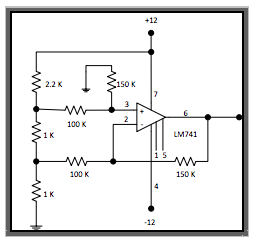
\includegraphics[width = 8cm, height = 5cm]{c5.png}
\centering \linebreak \linebreak Figure 3.5.0: Subtracting Amplifier circuit.
\end{figure} \hfill

Finally the measured voltages were registered in table 6: \hfill \break

\begin{center}
\begin{tabular}[.5cm]{c c c}
\toprule
\toprule
\hspace{60pt} $V_{1}$ \hspace{60pt} & \hspace{60pt} $V_{2}$ \hspace{60pt} & \hspace{60pt} $V_{o}$ \hspace{60pt}  \\
\midrule
\midrule
5.7 V & 2.86 V & 4.3 V \\
\bottomrule
\linebreak
\end{tabular}
\linebreak Table 6: Voltage measured values.
\end{center} \hfill
